\section{Context: why imitating these books is a losing design}
\label{sec:funds}

A descriptive base rate disciplines every 13F strategy discussion.
Across 1{,}597 large filers ($\ge\$1$B disclosed book,
coverage-eligible, 2013--2026), the median frozen-book excess return
against the S\&P~500 is $\mathbf{-3.3\%}$ \textbf{per year before
fees}; only 13\% of funds have a positive information ratio, and the
best IR in the universe is $\approx 1.0$. Skill persistence ---
the rank correlation of information ratios between the sample's
halves --- is $+0.25$: real but far below what manager selection
requires, and the measured root cause of the entire smart-money
graveyard (Section~\ref{sec:laws}).

The composition arithmetic matters more than the skill statement. The
cap-weighted index self-concentrates into its winners, and over this
sample a handful of mega-caps generated most of the index return
while the median stock lagged far behind \citep{bessembinder2018}.
Any portfolio more diversified than cap-weight --- and every 13F
book is, by mandate, liquidity, or prudence --- carries an
equal-weight tilt that this regime taxed structurally. The group
sorts photograph the tax directly: 27-name books lose $3.2\%$/yr
with 24\% positive-IR, while 790-name books sit at 1\%; true active
share is monotone in IR; turnover sorts favor the active. Two design
conclusions follow. A long-only-versus-S\&P imitation strategy is
condemned by arithmetic before any signal question arises. And the
alpha in this dataset lives not in the books but in the \emph{flows
and constraints between managers} --- fresh conviction and forced
selling --- exactly where the funnel found it. Caveats stated: the
disclosed book is long-only (no shorts, cash, or intra-quarter
turnover), and survivorship biases the level upward.

\begin{figure}[t]
\centering
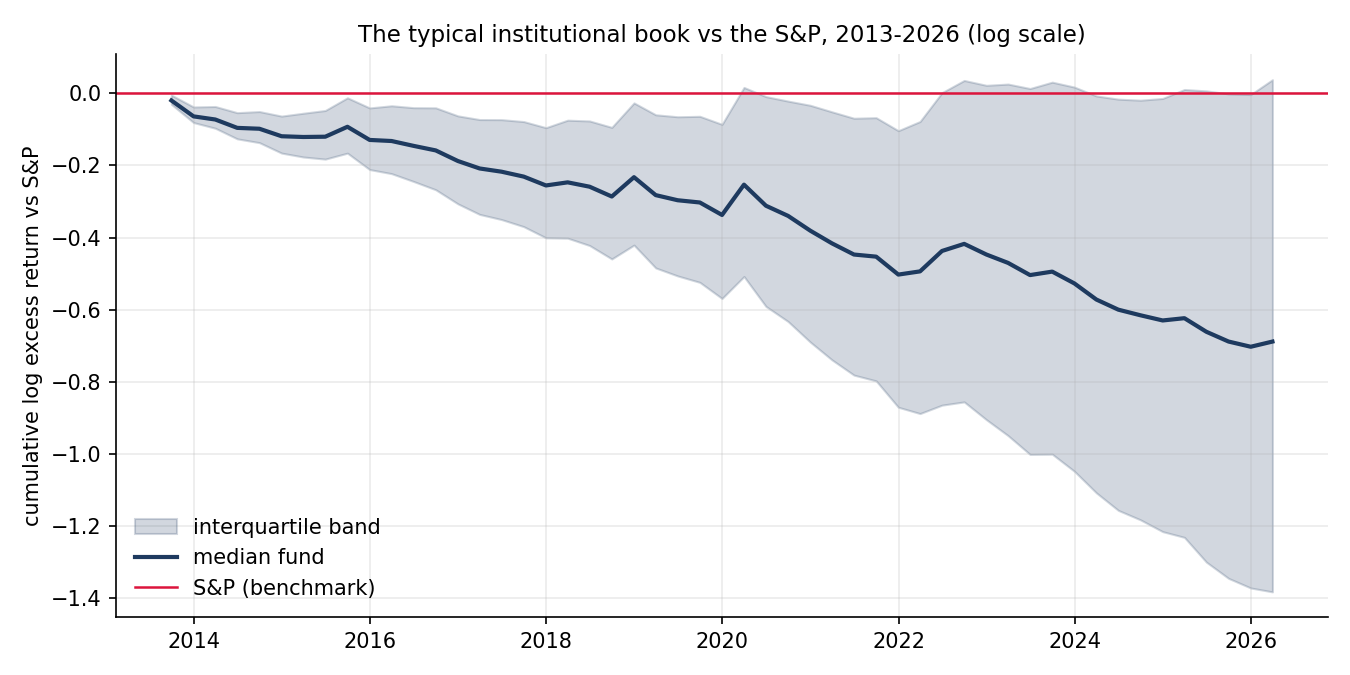
\includegraphics[width=.9\linewidth]{figs/funds_cum_log_excess.png}
\caption{Cumulative log excess return versus the S\&P~500 of large
13F filers (median and quantile bands): the median large
institutional book loses steadily against the index before fees.}
\label{fig:funds}
\end{figure}

\begin{figure}[t]
\centering
\begin{minipage}{.48\linewidth}
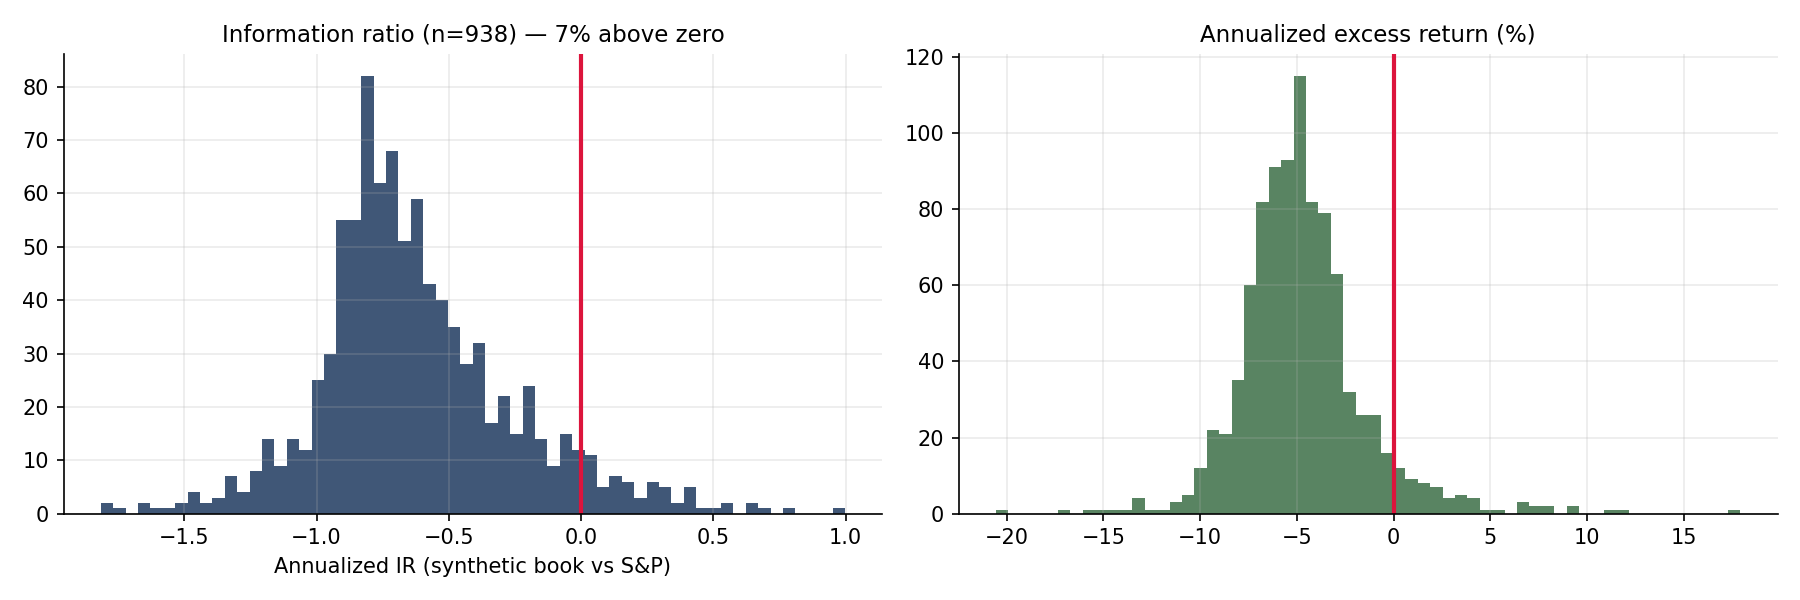
\includegraphics[width=\linewidth]{figs/funds_ir_histogram.png}
\end{minipage}\hfill
\begin{minipage}{.48\linewidth}
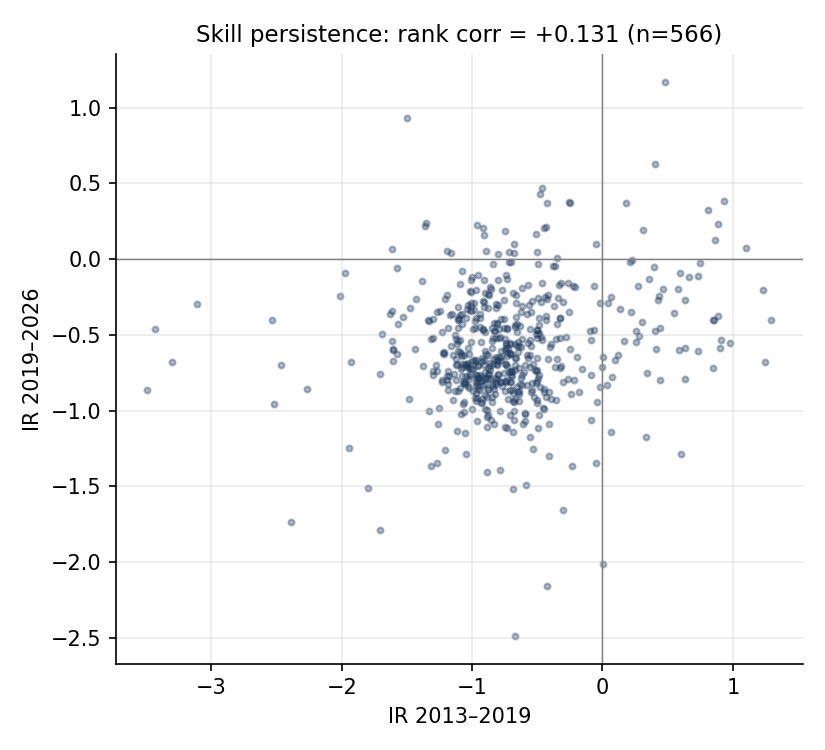
\includegraphics[width=\linewidth]{figs/funds_persistence.png}
\end{minipage}
\caption{Left: information-ratio distribution across 1{,}597 large
filers --- 13\% positive, best $\approx 1.0$. Right: skill
persistence (IR rank, first vs second half): $+0.25$, the measured
root of the smart-money graveyard.}
\label{fig:funds2}
\end{figure}
